\documentclass[conference, 11pt]{IEEEtran}
\IEEEoverridecommandlockouts

\usepackage{amsmath,amssymb,amsfonts}
\usepackage{algorithmic}
\usepackage{graphicx}
\usepackage{textcomp}
\usepackage{xcolor}
\usepackage{hyperref}
\usepackage{caption}
\usepackage[
    backend = biber,
    language = auto,
    style = numeric,
    sorting = none,
    block = space,
    hyperref = true,
    bibencoding = auto,
    giveninits = true,
    doi=false,
    isbn=false,
    alldates=short
]{biblatex}
\addbibresource{literature.bib}

\captionsetup{justification=centering,margin=0.5cm}

\def\BibTeX{{\rm B\kern-.05em{\sc i\kern-.025em b}\kern-.08em
    T\kern-.1667em\lower.7ex\hbox{E}\kern-.125emX}}
\begin{document}

\title{3DCV - Critical Driving Scenarios\\
{\small Generate critical driving scenarios in CARLA simulator and apply imitation learning to train a neural network}
}

\author{
    \IEEEauthorblockN{Christopher Klammt}
    \and
    \IEEEauthorblockN{Tobias Richstein}
    \and
    \IEEEauthorblockN{Julian Seibel}
    \and
    \IEEEauthorblockN{Karl Thyssen}
}

\maketitle

\begin{abstract}
	In this project report, we present an approach for generating new scenarios for supporting autonomous driving tasks in critical situations using the CARLA simulator along with it's Scenario-Runner. Our approach consists of generating new XML-based OPENScenario files which can be interpreted by the Scenario-Runner. Based on already present basic Scenarios, we apply a variety  of changes to attributes which are crucial for different sensors of an autonomous car. We considered external factors like weather, road conditions, time of day, color and models of cars, cyclists and pedestrians. In a second step, we transform the scenarios to different places in the same town and to different towns. To ensure the novel generated scenarios are valid, we consider different sanity checks as well as a specific verification to avoid duplicating scenarios.
	Also, we use the generated scenarios for training a model using imitation learning. TODO..

\end{abstract}

\begin{IEEEkeywords}
CARLA simulator, Scenario generation, Critical driving scenarios, Imitation learning, Autonomous driving
\end{IEEEkeywords}

\section{Introduction}
Autonomous driving vehicles are not just an idea for the more distant future, but rather a very current topic.
Not only Tesla, the company that dominates the news in this regard, is showing how far autonomous driving has come in the last years.
One crucial issue still lies in providing a stable and safe behavior in critical situations, especially in which traffic participants behave unexpectedly. 
The problem is that to robustly learn the appropriate behavior for these specific critical scenarios and to generalize using supervised learning a large amount of training data is needed.

In order to tackle this problem, our paper describes the development of a generator for such critical driving scenarios in the CARLA simulator.
These critical driving scenarios are mainly inspired by the report \citetitle{NHTSA:PreCrashScenarios} \cite{NHTSA:PreCrashScenarios} for the National Highway Traffic Safety Administration in the United States.
These contain scenarios such as avoiding an obstacle, lane changing with oncoming traffic or crossing traffic running a red light at an intersection (as shown in \autoref{fig:scenario-run_red_light}).

\begin{figure}[ht]
    \centering
    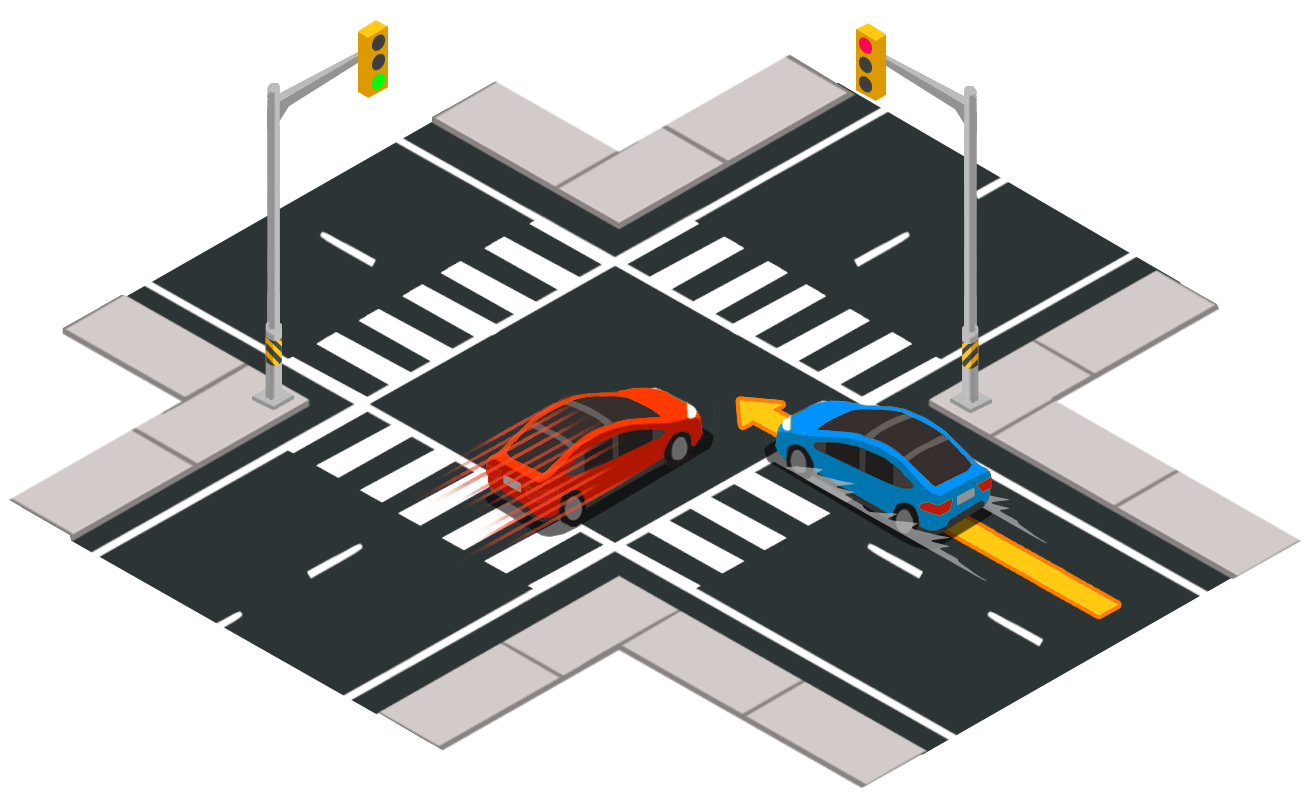
\includegraphics[width=0.7\linewidth]{figures/scenario-run_red_light.png}
    \caption{NHTSA scenario: Crossing traffic running a red light at an intersection \cite{CARLAChallenge:Scenarios}}
    \label{fig:scenario-run_red_light}
\end{figure}

Furthermore, after generating these different critical driving scenarios we utilize them to learn a robust model.
To do so imitation learning is used, in which an expert demonstrates the desired behavior in each critical situation and is then adopted by the model.

\section{Related Work}

\subsection{CARLA}
As presented by \citeauthor{Dosovitskiy17:CARLA}, CARLA is an open-source urban driving simulator for autonomous driving research \cite{Dosovitskiy17:CARLA}.
It enables handling different use cases within the general problem of driving, such as learning driving policies or training perception algorithms.
To control the simulation, e.g. changing weather, adding cars or pedestrians, an API is available in Python and C++.
CARLA consists of the simulator responsible for rendering etc. as well as multiple components, for example a traffic manager controlling the vehicles or a component handling the sensors.

\subsection{Critical driving scenarios}

Another component that works in unison with the CARLA simulator is the ScenarioRunner \cite{CARLA:ScenarioRunner}.
This is a module that makes it possible to define various traffic scenarios and execute them in the CARLA simulator.
These scenarios can be defined using Python or the OpenSCENARIO \cite{OpenScenario} standard.
The ScenarioRunner already contains some predefined Scenarios which are based on the critical driving scenarios as described in \citetitle{NHTSA:PreCrashScenarios} \cite{NHTSA:PreCrashScenarios}.

\subsection{Generating data in simulators}

In order to generate data it first is necessary to identify parameters that are to be adjusted and that should vary across the different entities.
The data generation can then be approached in different ways.
One possibility is to use a random statistical distribution of these parameters. 

Another way to go about data generation is to use learning-based methods to adjust the parameters of the simulator.
Such an approach was chosen by \citeauthor{DBLP:LearningToSimulate} and published in \citetitle{DBLP:LearningToSimulate} \cite{DBLP:LearningToSimulate}.
They proposed a reinforcement learning-based method to adjust the parameters of the synthesized data to maximize the accuracy of a model trained on that data.
A quite similar approach was chosen by \citeauthor{DBLP:Meta-Sim} \cite{DBLP:Meta-Sim} called Meta-Sim, which learns a generative model of synthetic scenes and modifies the attributes using a neural network.

\subsection{Imitation learning}

To learn a model based on labeled data some form of supervised learning is generally applied.
\citeauthor{Chen:LearningByCheating} propose a method called \citetitle{Chen:LearningByCheating} \cite{Chen:LearningByCheating}.
This is a two-stage method, in which first an agent is trained using privileged information.
In the second stage, the privileged agent acts as a teacher that trains a purely vision-based agent.

Another approach is \citetitle{Toromanoff_2020_CVPR} \cite{Toromanoff_2020_CVPR}. Here reinforcement learning is utilized to learn an optimal behavior policy based on a reward-function, effectively punishing wrong behavior such as leaving the track or running over pedestrians.

To train and manage the trainings of imitation learning networks jointly with evaluations on the CARLA simulator \citetitle{felipecode:coiltraine} \cite{felipecode:coiltraine} can be used.

\section{Method}

\subsection{Generating new scenarios through ScenarioRunner}
In general, we identified the two possible ways to create new scenarios that are supported by the ScenarioRunner.
The first option consists of using the Python based API of the ScenarioRunner library to define the dynamic behavior of every actor in combination with a \texttt{xml}-based configuration file, which can be used to initialize different parameters for a predefined python based scenario.

The second option is to utilize  OpenSCENARIO-based configuration files supported by the ScenarioRunner. OpenScenario is standard \texttt{xml}-based file format for the description of dynamic contents in driving simulation applications \cite{OpenScenario}. These configuration files differ from the former approach mainly in one aspect. For defining OpenSCENARIO based scenarios, there is no need to create the python-based scenario description. Therefore OpenSCENARIO can be used to generate all configurations for executing a scenario through the ScenarioRunner library at once. 

Both the introduced options come with advantages and disadvantages. For our decision process, we identified three criteria which we would expect for the approach we want to work with. 
The first criteria is  \textit{generalization}. We would expect that the approach can be well generalized by extracting an abstract process which can be applied to all the different formats a new scenarios could possibly have.
The second criteria is \textit{the number of directly  accessible and adjustable parameters}. Since we aim to provide a scenario generation process which is capable of generating as many scenarios as possible, we want to achieve a high number of adjustable parameters for providing a large combinatoric basis.
The third and last criteria we considered is \textit{simplicity} of the overall concept. Reducing the complexity and  following the KISS (Keep it simple, stupid)-Principle for achieving different advantages in further developments like extensions and maintenance. 

Finally after evaluating both the options for generating new scenarios with respect to the defined criteria, we concluded to use the OpenSCENARIO-based approach. Overall we saw only advantages by using the openSCENARIO standard as our final way for generating new scenarios. In comparison to the Python-based scenario generation, openSCENARIO can be better generalized in terms of generating the files itself. It is pretty uncommon and connected with more effort to generate Python-files for setting up scenarios. In addition, the \texttt{xml} configuration needs to be generated as well. OpenSCENARIO-based files are including all the necessary data combined in one file, which is additionally \texttt{xml}-based. Therefore it provides an easy file-generation while maintaining all the information for one scenario. Considering the second criteria of direct accessible and adjustable parameters, with OpenSCENARIO-files, all possible parameters which are crucial for a scenario are direct accessible and values can be changed easily.
All the described differences can be transferred to the last and third criteria of following the KISS-principle. It might be that a OpenSCENARIO file alone has a more complex structure, but nevertheless, it would be much more complicated to generate generic Python-files for defining new Scenarios.

\subsection{Design and Implementation}
With the decision of using OpenSCENARIO-files, we designed a generator tool which is capable of changing a variety of parameters that are decisive for the underlying problem of critical driving scenarios. Our approach utilizes the already present basic scenarios for critical driving situations of the ScenarioRunner. Since it is of tremendous effort to generate scenarios which state a completely new critical situation by changing the overall behavior of all actors, we first decided to use the five predefined scenarios, which will be called \textit{basic scenarios} in the further course of this report. Those include situations of a crossing bicycle,  changing weather conditions, following a leading vehicle, pedestrian crossing as well as a lane changing scenario.

We consider a scenario as new, if a single parameter value differs from all of the already generated scenarios. With this definition we can generate thousands of new scenarios by providing one base scenario.

To generate new values for selected parameters, we use the schema file for openSCENARIO-files of CARLA which comes along with the ScenarioRunner tool. We extract mainly attribute names of tags we considered changeable in the context of this project as well as their data-types and valid values if the data-type is categorical.

 Therefore we extract available information for example of the \texttt{<weather>}-tag, which has an attribute \texttt{cloudState} that only accepts values of a predefined enum type. Our generator would extract all possible values which is in the mentioned case a set of ["\texttt{free}", "\texttt{cloudy}", "\texttt{overcast}", "\texttt{rainy}", "\texttt{skyOff}"]. With the information of all attributes and their data-types and the basic scenario as template, new scenarios are generated. We also extract the information about the map, the scenario plays in. This is a prerequisite for extracting values of pedestrian and vehicle types from the CARLA Python API, since the valid and possible values of those attributes depend on the actual map.
 For all the tags which include attributes of categorical values we apply a random choice on all possible values. In the case of numeric attributes, we change the values based on the set values in a range of [-100\%, +100\%].
 For every base scenario which is accessible, the user can specify how many additional scenarios should be created. After every new scenario, we use a hash value based comparison on the document to execute a duplication check such that we avoid the generation of the exact the same scenario twice.
The overall generator-flow is shown in figure \ref{fig:generator-flowchart}.

TBD:
 Attribute tree 

\begin{figure}[ht]
	\centering
	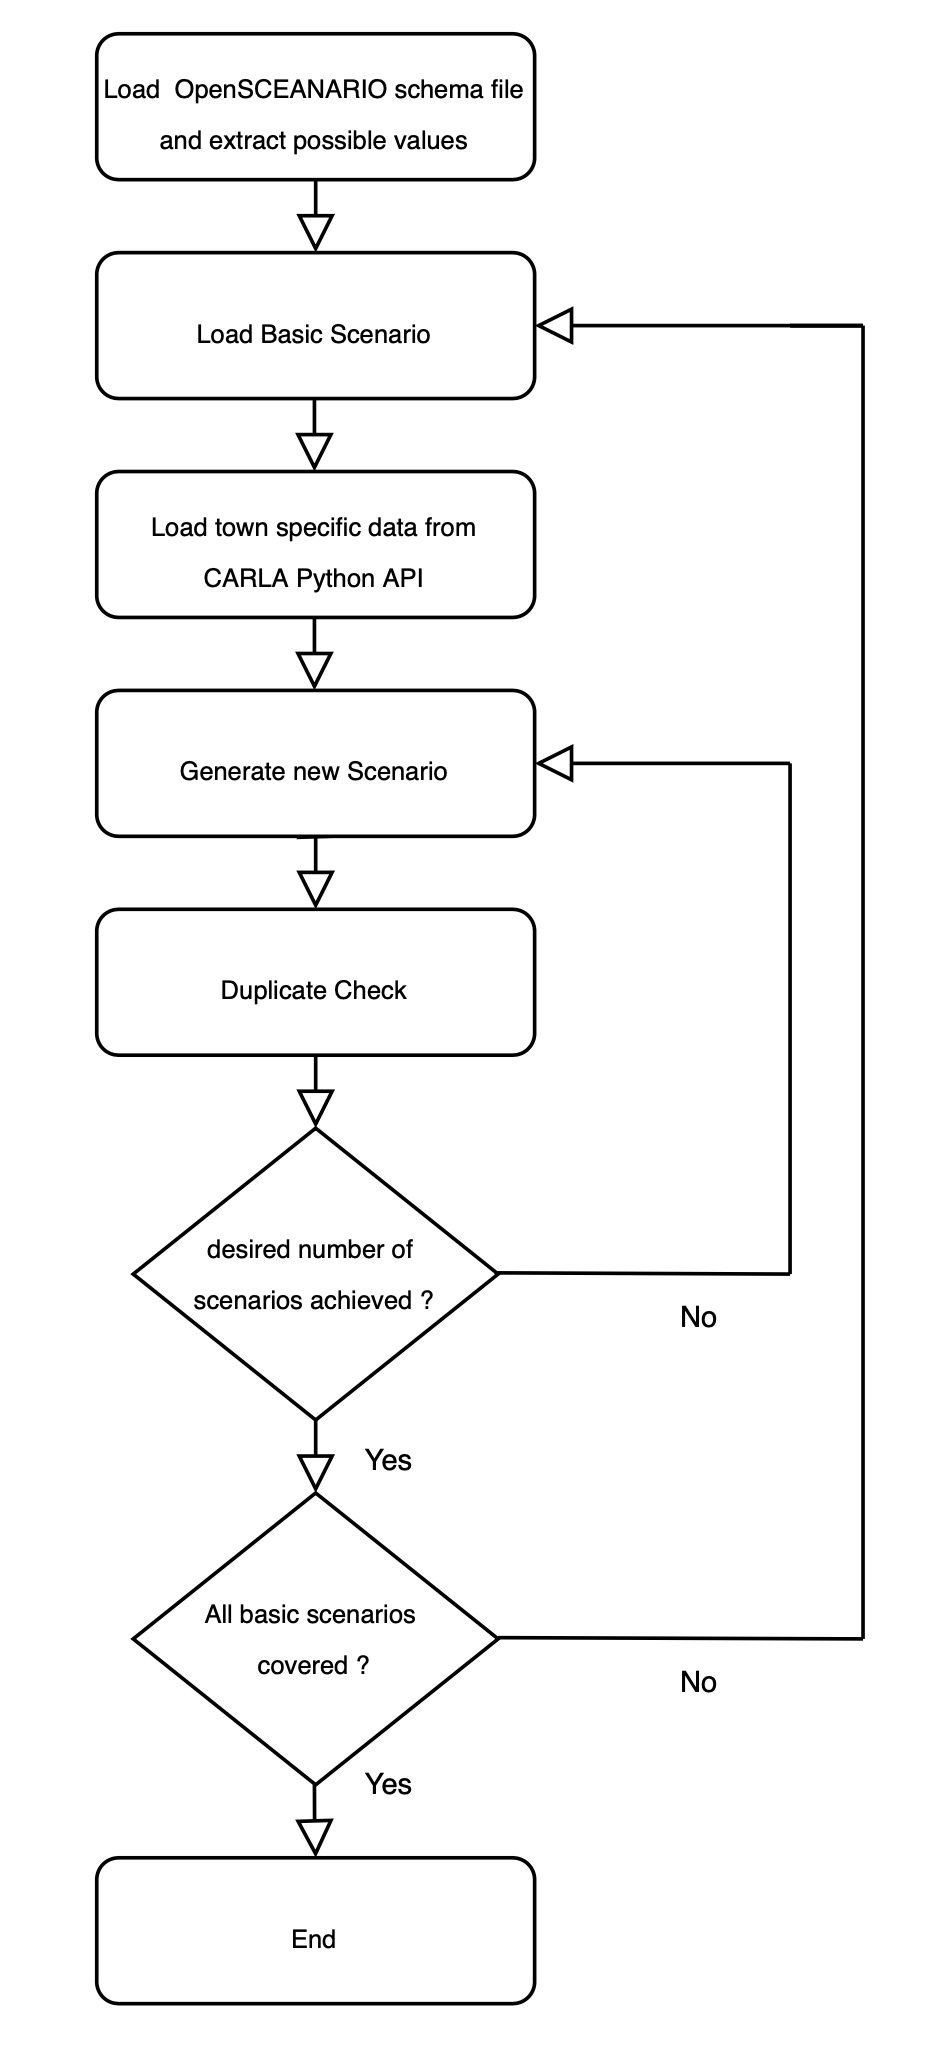
\includegraphics[width=0.9\linewidth]{figures/generator-flow.png}
	\caption{Flow-Chart of the scenario-generator.}
	\label{fig:generator-flowchart}
\end{figure}

\subsection{Adjustable parameters}

CARLA and the ScenarioRunner enable us to adjust quite a few parameters, so that the generator can create a lot of diverse settings. In theory we have access to all possible parameters by the ScenarioRunner tool which are contributing to a single scenario. Since most of them are interventions into the semantics of a scenario, we propose to first change parameters which are not changing the overall actor behavior.
This includes the type and model of the car, which is steered by the learned agent, but more importantly of each and every other car.
This is important so that the model generalizes well, even if cars of different size, shape and color are in it's field of vision resulting in different RGB patterns perceived by the cars sensors.
Another parameter, that can be changed is the speed of the cars, which also has an impact on the behavior in critical situations.
This setting is not limited to cars, also available bicycle and pedestrian types are used in similar manner.

Moreover the weather plays an important role, as it drastically changes what is perceived by sensors and also alters the effects of a certain behavior. For example precipitation does not only impair the video of the camera, but additionally lengthens the breaking distance.
These variables can all be adjusted rather easily, by just randomly picking a value from the set of possible values.
Similar, we are feasible of adjusting all available attributes for sun and fog tags.

In addition, we generate a random time of day for every new scenario to cover also an increasing danger in situations for example in night, where pedestrians and bicycles are harder to detect.

To also simulate a variety of different road conditions, we include a random generated friction scale factor for every new scenario. Those factors can be influenced by many external effects like oil spilled on the road.

However, these attributes are independent from the original spawn-position of all actors. As an additional requirement, the generation of new scenarios should include a relocation of the scene to another suitable place in 
the same map or even in a different map.
For this, we first analyze the initial situation by fetching the closest town specific waypoints based on the initial actor position. To get information about the scenario circumstances we use a simple approach to detect whether the scenario takes place on a intersection by calculating and comparing the distances between the actors and the hero (ego-vehicle) actor to the next intersection in driving direction. If the latter distance is less, we conclude that the scenario must take place at an intersection. This information is valuable for shifting the scenario to another  position in the same or different town. We do this with respect to all the conditions given by the initial scenario for instance retaining distances between all actors.

If we conclude that the scenario takes place at an intersection, we fetch all possible junctions using the Python API of CARLA for a specific map. The closest junction in driving direction is used  as the scenario anchor. 

For some scenarios, it is typical that actor positions like for pedestrians or cyclists are not considered as waypoints since they spawn off-road.  If we detect such a deviation we calculate a offset between the actual actor position and the nearest waypoint. To apply the correct orientation we rotate the position of the actor with respect to the new orientation of the road.

\begin{equation}
	M = \left(\begin{matrix} cos(\alpha) & sin(\alpha) \\ - sin(\alpha) & cos(\alpha) \end{matrix}\right) *  \left(\begin{matrix} x \\ y \end{matrix}\right) 
\end{equation}

tbd. picture of bike scenario + mit distancen

Not all positions calculated will work on different maps. Therefore we include two sanity checks when calculating new actor positions. 

The part of the configuration, which is more difficult to vary is with regards to further actors, such as pedestrians and other vehicles.
These have to be spawned somewhere and a behavior needs to be defined.
CARLA provides a list of possible spawn points across a specific map, but if we just choose these randomly, we cannot be sure, that the spawned car has an impact on our scenario.
Most importantly, the behavior of the car, which characterizes the critical scenario needs to well defined.
But apart from that, we also want vehicles in the background, that drive around somewhat automated.

\subsection{Limitations}
Kein Einfluss auf Autopilot route, nicht deterministisch. Pro intersection gibt es Wahrscheinlichkeiten die zum Moment nicht beeinflussbar sind. Eigentliche Route kann vom Agent geplant werden.

+ problems faced:
\begin{itemize}
	\item Keine semantische informationen  bei scenarios
	\item nur 5 basis scenarien, um komplett neue situationen zu definieren, müssten neue basis scenarien generiert werden.
	\item ...
\end{itemize}

\subsection{Imitation Learning Approach}
tbd,.

\section{Experiments}
tbd. 



\section{Conclusion}
To conclude this report, we try to answer three research questions based on the outcome of our experiments.

• Can we generate critical scenarios such that a model trained
on these scenarios achieves robustness against critical
scenarios?

• How many critical scenarios have to be represented in the
training distribution in order to achieve robustness against
critical scenarios?

• Does robustness against a certain type of critical scenario
transfer to a different type of critical scenario?

\printbibliography

\end{document}
